\chapter{K邻近模型}

\section{懒惰的想法:少数服从多数}

假设说我们有一堆玩具,分别是加号,减号,和三角形,其中还有一个被隐藏住看不清形状,我们要判断一个不能确定形状的玩具到到底是三角形,
还是长方体,根据薛定谔的猫原理,你在没有观测到最它那当然加号减号三角形三个状态同时存在(不是QWQ),但是现实问题是我们只能选择一个可能
,那最懒惰的方法就是:\textsl{看三种类型的玩具哪个出现的频次最多,我就认为这个未知的就是哪种类型。}

\begin{figure}[H]
    \centering
    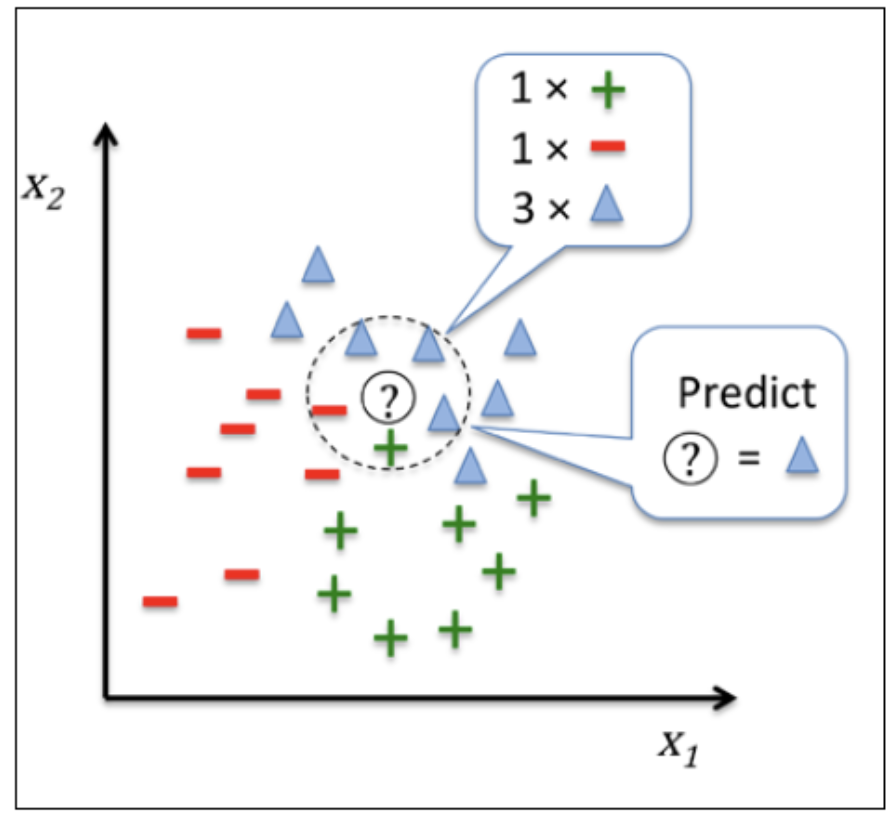
\includegraphics[scale=0.2]{figures/k-nearest.png}
    \caption{判断小球属于哪一类?}
\end{figure}

但是一下子统计所有玩具太累人了,干脆选一个小区域吧,反正就算统计完所有玩具,认为它是出现最多的那种类型也不一定对,就选一个小区域随便
定一下就好了,所以如上图所示,我们画了一个小圈,小圈里有三个三角形,一个加号一个减号,所以我们预测这个未知的类型是三角形。这就是$k
$邻近算法的思想,对于机器学习来说就是:\textsl{以需要预测的点为中心划分一个区域,判断区域内所有出现次数最多的类型,认为未知的类型就是
出现次数最多的}。
\section{距离的度量}

设特征空间$\mathcal{X}$是$n$维实数向量空间$\mathbb{R}^n$,$x_i,x_j\in \mathcal{X}$,其中$x_i=(x^{(1)}_i,x^{(2)}_i,\cdots,x^{(n)}_i)^T$,
$x_j=(x^{(1)}_j,x^{(2)}_j,\cdots,x^{(n)}_j)^T$,则$x_i,x_j$的\textbf{$L_p$距离}定义为
\begin{equation}
    L_p(x_i,x_j)=\left(\sum_{l=1}^{n}|x^{(l)}_i-x^{(l)}_j|^p\right)^{\frac{1}{p}}
\end{equation}

当$p=2$时,那就是\textsl{欧几里得距离(Euclidean distance)}
\begin{equation}
    L_2(x_i,x_j)=\sqrt{\left(\sum_{l=1}^{n}|x^{(l)}_i-x^{(l)}_j|^2\right)}
\end{equation}

当$p=1$时,称为\textsl{曼哈顿距离(Manhattan distance)},即
\begin{equation}
    L_1(x_i,x_j)=\sum_{l=1}^{n}|x^{(l)}_i-x^{(l)}_j|
\end{equation}

当$p=\infty$时,它是各个坐标距离的最大值
\begin{equation}
    L_{\infty}(x_i,x_j)=\max\limits_{l} |x^{(l)}_i-x^{(l)}_j|
\end{equation}

下图描述二维空间中$p$取不同值时,与原点的$L_p$距离为$1$的点的关系
\begin{figure}[H]
    \centering
    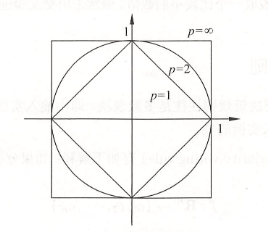
\includegraphics[scale=0.7]{figures/LP距离之间的关系.png}
    \caption{$L_p$距离之间的关系}
\end{figure}

\section{k邻近算法}

\begin{framed}
    \textbf{算法:(k邻近法)}

    输入:训练数据集$T=\{(x_1,y_1),(x_2,y_2),\cdots,(x_N,y_N)\}$,其中$x_i\in \mathcal{X}\subseteq \mathbb{R}^n$为实例的特征向量,$y_i\in \mathcal{Y}=\{c_1,c_2,\cdots,c_K\}$
    为实例类别;

    输出:实例$x$所属类别$y$.

    \begin{enumerate}[itemindent=2em]
        \item 在训练集$T$中找出与$x$最邻近的$k$个点,函盖$k$个点的$x$的邻域记作$N_k(x)$;
        \item 在$N_k(x)$中根据分类决策规则决定$x$的类别$y$;
    \end{enumerate}
    \begin{equation}
        y=\arg\max\limits_{c_j}\sum_{x_i\in N_k(x)} I(y_i=c_j),\ \ \ i=1,2,\cdots,N,\ \ j=1,2,\cdots,K
    \end{equation}
\end{framed}

$k$等于1时,称为\textsl{最邻近算法}。

\section{空间划分:kd tree}

实现$k$邻近算法时,主要考虑的问题是如何对训练数据集进行快速$k$邻近搜索。

\subsection*{kd树构造}

构造\textsl{kd tree}相当于不断地用垂直于坐标轴的超平面将$k$维空间划分,构成一系列的$k$维超矩形区域。

\begin{framed}

    \textbf{算法:(kd-tree构建)}

    输入:训练数据集$T=\{x_1,x_2,\cdots,x_N\}$,$x_i=\{x^{(1)}_i,x^{(2)}_i,\cdots,x^{(k)}_i\}$
    为实例类别;

    输出:KD tree.

    \begin{enumerate}[itemindent=2em]
        \item 开始:构造根节点,跟节点对于包含$T$的$k$维空间的超矩形区域;
        
        选择$x^{(l)}$为坐标轴,以$T$中所有实例$x^{(l)}$坐标的中位数为切分点,将根节点对应的超矩形区域切分为两个子区域,切分由通过切分点并与坐标轴$x^{(l)}$垂直的超平面实现。

        \item 重复:对深度为$j$对节点,选择$x^{(l)}$为切分的坐标轴,$l=j(mod\ k)+1$,以该结点的区域中所有的实例的$x^{(l)}$,
        以该结点的区域中所有的实例的$x^{(l)}$坐标的中位数作为切分点,将该结点对应的超矩形区域切分为两个子区域。切分由通过切分点并
        与$x^{(l)}$垂直的超平面实现。

        由该节点生成的深度为$j+1$的左右子节点;左子节点对应坐标$x^{(l)}$小于切分点的子区域,右子节点对应的坐标$x^{(l)}$大于切分点的子区域。
        将落在切分超平面上的实例点保存在该节点。

        \item 直到两个子区域没有实例存在则停止划分;

    \end{enumerate}

\end{framed}

\begin{figure}[H]
    \centering
    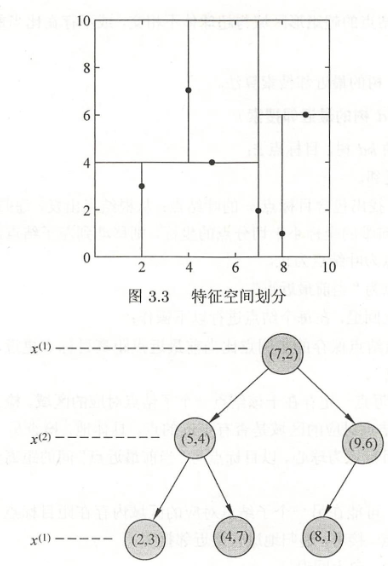
\includegraphics[scale=0.5]{figures/kd-tree2.png}
    \caption{kd  tree实例}
\end{figure}

\subsection*{kd树搜索}

\begin{framed}

    \textbf{算法:(kd-tree构建)}

    输入:kd tree;

    输出:x的最邻近.

    \begin{enumerate}[itemindent=2em]
        \item 在\textsl{kd tree}中赵处包含目标点$x$的叶子结点,从根节点出发,递归地向下访问,若目标点当前维的坐标小于切分点坐标,则移动到左子节点,否则移动叶子结,直到子节点为叶结点为止。
        
        \item 以此叶子结点为当前最近点;
        \item 递归向上回退,在每个结点进行以下操作:
        \begin{enumerate}
            \item 如果该结点保存的实例点比当前最近点距离目标点更近,则以该实例点为“当前最近点”;
            \item 当前最近点一定存在一个该结点一个子结点对应的区域,检查该子结点的父结点的另一子结点对应的区域是够有更近的点,具体地,检查另一子结点对应的区域是否以目标点为球心,以目标点与“当前最近点”间距离为半径的超球体相交;
            
            如果相交,可能在另一个子结点对应的区域内存在距离目标点更近的点,移动到另一子结点,接着,递归进行最邻近搜索;如果不相交,则向上回退;
            \item 当回退到根结点时,搜索结束,最后的当前最近点即为$x$的最邻近点。
        \end{enumerate}

    \end{enumerate}

\end{framed}

\subsection*{实例}

\begin{figure}[H]
    \centering
    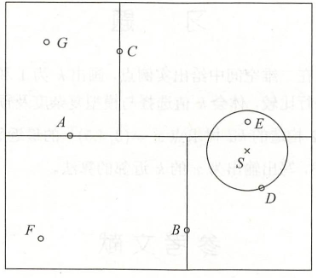
\includegraphics[scale=0.5]{figures/kd-tree-ex.png}
    \caption{kd  tree搜索实例}
\end{figure}

首先找到包含$S$的叶子结点$D$,以$D$为近似最邻近,真正的最邻近一定是以$S$为中心通过点$D$的圆的内部,然后返回节点$D$的父结点$B$,
在$B$的另一子结点$F$的区域内搜索最邻近。结点$F$的区域与圆不相交,不可能有最邻近点;继续返回上一级父节点$A$,在结点$A$的另一子结点$C$
的区域内搜索最邻近,结点$C$与圆相交,该区域内有实例点$E$,点$E$比$D$更近,成为新的最邻近点,最后得到$E$是$S$的最邻近。

\subsection*{处理维数灾难}

维数灾难让大部分的搜索算法在高维情况下都显得花俏且不实用。 同样的,在高维空间中,$kd$树也不能做很高效的最邻近搜索。一般的准则是:在k维情况下,数据点数目N应当远远大于
$2^k$时,$kd$树的最邻近搜索才可以很好的发挥其作用。不然的话,大部分的点都会被查询,最终算法效率也不会比全体查询一遍要好到哪里去。另外,如果只是需要一个足够快,且不必最优的结果,那么可以考虑使用近似邻近查询的方法。